% Source: graduate-coursework/Sp26/CSCE763/Course_Assignments/HW1/HW1_CSCE_763_solutions.tex

\documentclass[border=4pt]{standalone}
\usepackage{amsmath}
\usepackage{amssymb}
\usepackage{graphicx}
\usepackage{tikz}
\usepackage{xcolor}
\usetikzlibrary{shapes.geometric, arrows.meta, positioning, patterns}

\definecolor{USC_Garnet}{HTML}{73000A}
\definecolor{USC_Sandstorm}{HTML}{FFF2E3}
\definecolor{USC_Black90}{HTML}{363636}
\definecolor{USC_Black70}{HTML}{5C5C5C}
\definecolor{USC_Black50}{HTML}{A2A2A2}
\definecolor{USC_Black10}{HTML}{ECECEC}
\definecolor{USC_Honeycomb}{HTML}{65780B}
\definecolor{USC_Atlantic}{HTML}{466A9F}
\definecolor{USC_Congaree}{HTML}{1F414D}
\definecolor{USC_Rose}{HTML}{CC2E40}
\definecolor{outputbg}{RGB}{245,245,245}

\begin{document}
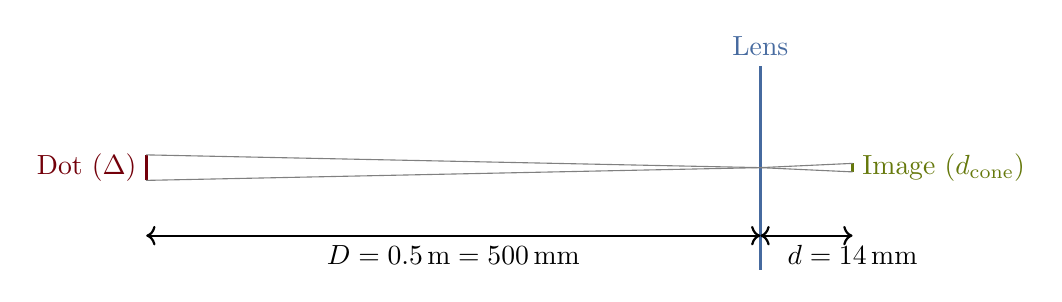
\begin{tikzpicture}[xscale=1.95, yscale=1.08]
    % Lens
    \draw[thick, USC_Atlantic] (4, -1.2) -- (4, 1.2);
    \node[above, USC_Atlantic] at (4, 1.2) {Lens};

    % Object (dot)
    \draw[very thick, USC_Garnet] (0, -0.15) -- (0, 0.15);
    \node[left, USC_Garnet] at (0, 0) {Dot ($\Delta$)};

    % Image (on retina)
    \draw[very thick, USC_Honeycomb] (4.6, -0.05) -- (4.6, 0.05);
    \node[right, USC_Honeycomb] at (4.6, 0) {Image ($d_{\text{cone}}$)};

    % Rays
    \draw[thin, gray] (0, 0.15) -- (4, 0) -- (4.6, -0.05);
    \draw[thin, gray] (0, -0.15) -- (4, 0) -- (4.6, 0.05);

    % Distance labels
    \draw[<->, thick] (0, -0.8) -- (4, -0.8);
    \node[below] at (2, -0.8) {$D = 0.5\,\text{m} = 500\,\text{mm}$};
    \draw[<->, thick] (4, -0.8) -- (4.6, -0.8);
    \node[below] at (4.6, -0.8) {$d = 14\,\text{mm}$};
\end{tikzpicture}
\end{document}
